
\begin{figure}[ht!]
    \centering
	\captionsetup{justification=justified, singlelinecheck=false, width=1\textwidth}
    \caption{Gráficos de completeza dos dados para as estações BC4, BC9 e BC12 durante o período do mês de maio.2023. O registro de todas as estações foi satisfatório durante o período. Para a estação BC4, os últimos dois dias não foram incluídos por problemas na transmissão dos dados para o IPT, entretanto, serão analisados e incluídos no relatório anual. }
    \begin{mdframed}[
        linecolor=black,
        linewidth=1pt,
        roundcorner=10pt,
    ]
    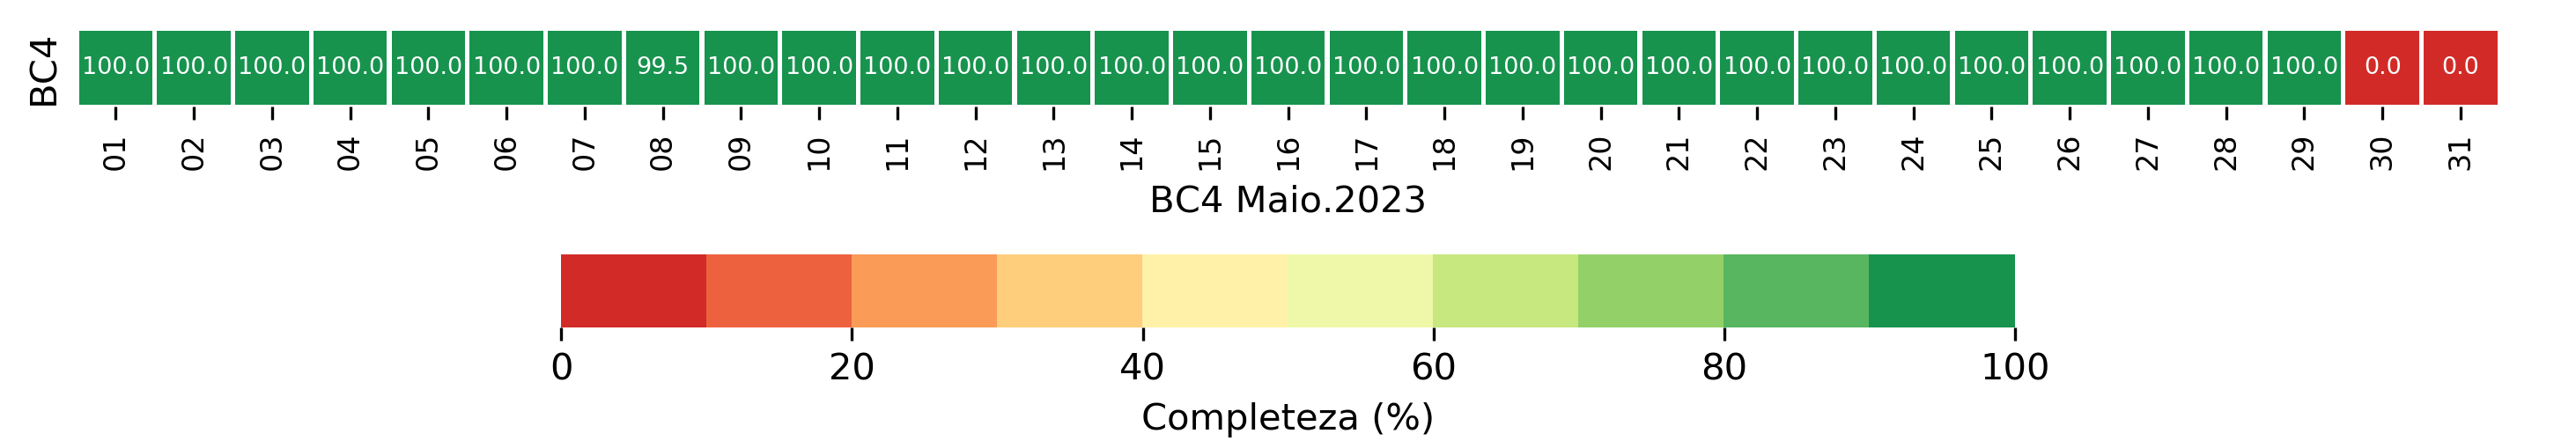
\includegraphics[width=1.0\textwidth]{./boletim/baesa/figuras/bc4_completude.png}
    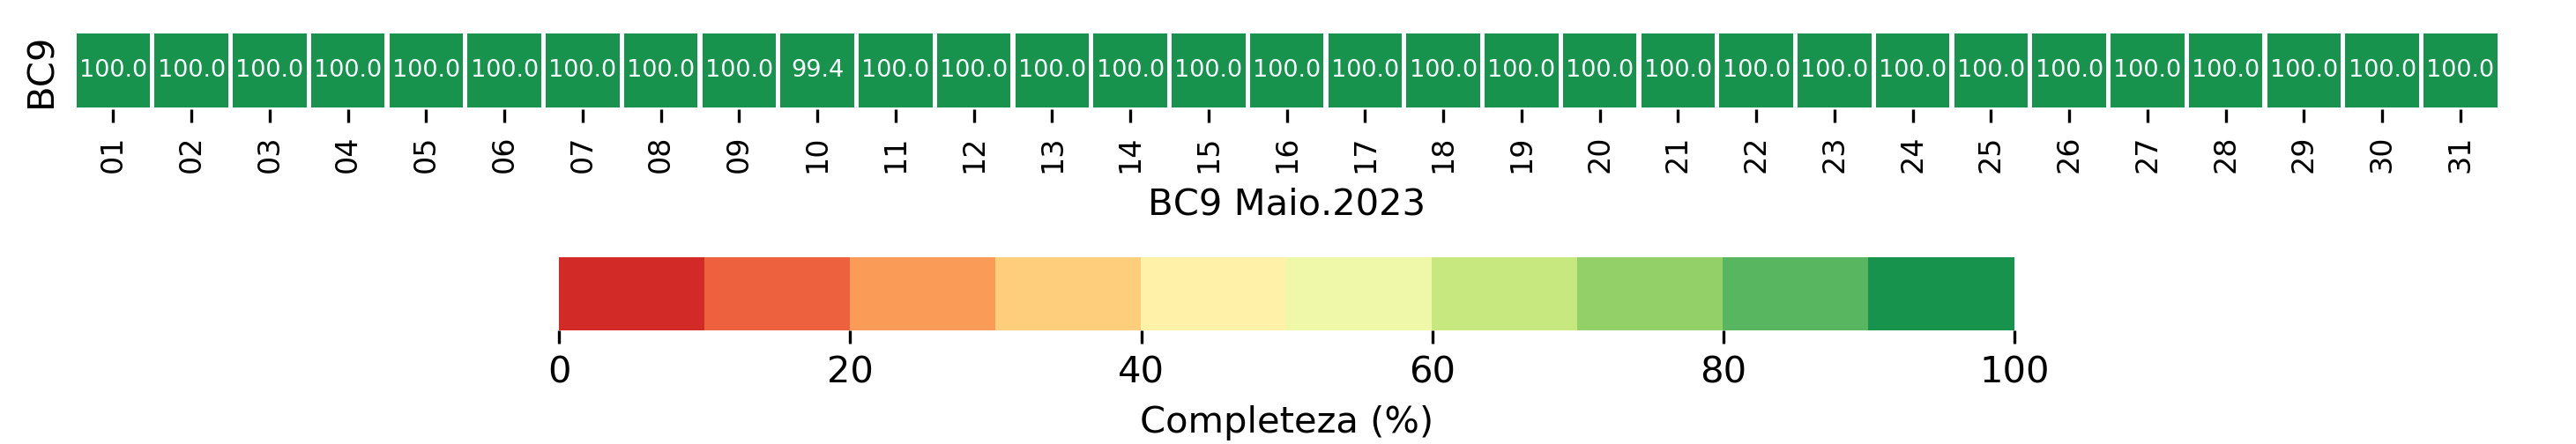
\includegraphics[width=1.0\textwidth]{./boletim/baesa/figuras/bc9_completude.png}
    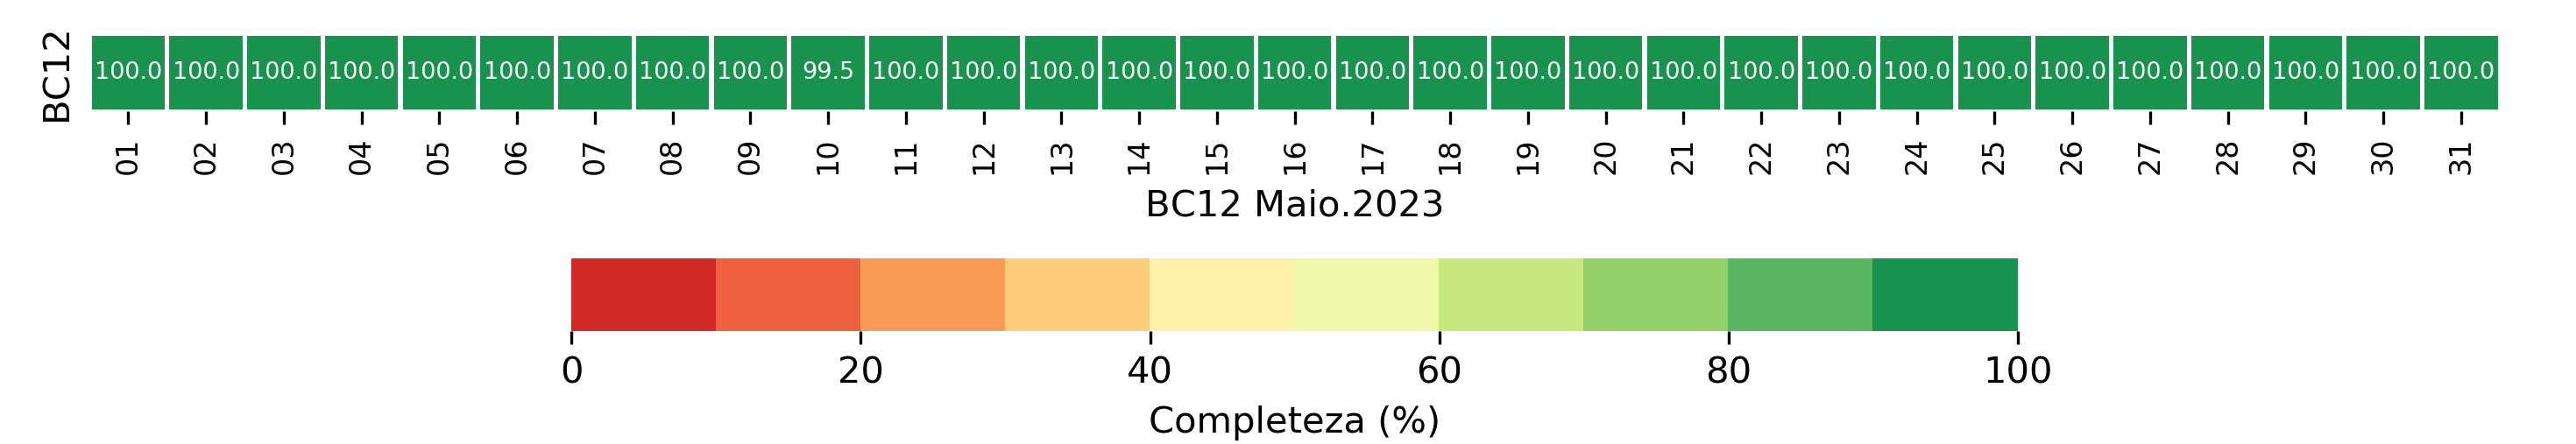
\includegraphics[width=1.0\textwidth]{./boletim/baesa/figuras/bc12_completude.png}
    \end{mdframed}
    \caption*{Fonte: IPT}
\end{figure}
